Six technical chapters have culminated to the main event, the numerical experiments and their results. This is where we learn if BNNs can deliver on the promise of substituting direct calculations of cross sections. We will begin with a description of the dataset and the data transformations made prior to training and their potential implications for the predictive performance of the trained BNNs. We will then explain the methodology employed including the implementation details, the selection of BNN models and hyperparameters and performance metrics. Once discussed, we will explore the results and their consequences.



\section{The Dataset}\label{sec:dataset}
In this section, we will give a brief description of the dataset. Moreover, we will discuss the data transformations prior to training and its implications on the accuracy of the predictions.

For the predictions presented in this chapter, we have restricted our investigations to use the dataset for a single particle process throughout. This will make it easier to compare the performance of BNNs across different configurations to better understand the strengths and weaknesses of the different choices made when training BNNs. 

\subsection{The Features and Targets}
We will focus on a particular neutralino-neutralino. Neuralinos are denoted by the symbol $\tilde{\chi}_i^0$ for $i = 1, 2, 3, 4$.
Each neutralino carries its own \textit{mass} $m_{\tilde{\chi}_i}$ and a set of \textit{mixing angles} $N_{ij}$. For each neutralino $i$, there are four mixing angles for $j = 1, 2, 3, 4$. The two possible cases of interest then would be a process with two identical neutralinos, in which case the input features are of the form
\begin{equation}\label{eq:neutralino_feat}
    x = (m_{\tilde{\chi}_i^0}, N_{i1}, N_{i2}, N_{i3}, N_{i4}),
\end{equation} 
or a process where there are two distinct neutralinos $i$ and $k$, such that the input features would have the form
\begin{equation}
    x = (m_{\tilde{\chi}_i}^0, N_{i1}, N_{i2}, N_{i3}, N_{i4}, m_{\tilde{\chi}_k^0},  N_{k1}, N_{k2}, N_{k3}, N_{k4}).
\end{equation}
The targets of the dataset are NLO cross sections of the form
\begin{equation}
    \sigma_{\tilde{\chi}_i^0 \tilde{\chi}_k^0} = \text{LO} + \text{NLO}.
\end{equation}
In our case we will focus on processes that results in $\tilde{\chi}_1^0\tilde{\chi}_1^0$, meaning the input features have the form in eq.~\eqref{eq:neutralino_feat}. The masses $m_{\tilde{\chi}_i^0}$ can take on both postive and negative values in the dataset. In figure \ref{fig:dataset_masses}, we show the NLO cross sections $\sigma_{\tilde{\chi}_1^0 \tilde{\chi}_1^0}$ projected onto the axis of masses $m_{\tilde{\chi}_1^0}$ and in figure \ref{fig:dataset_mixing_angles} we show their values projected onto the axes of the mixing angles $N_{1j}$ for $j=1,2,3,4$. 
Note in particular that the cross sections span several orders of magnitude which necessitates a data transformation to reliably perform regression analysis with the dataset. We can also note a few outliers most of which yield neglible cross section values, but we should be aware of that adverse effect of these can affect the trained BNN models. There is a certain asymmetry in some of the features as well, where there are largely more cross sections on the right side of 


\begin{figure}[h!]
    \centering
    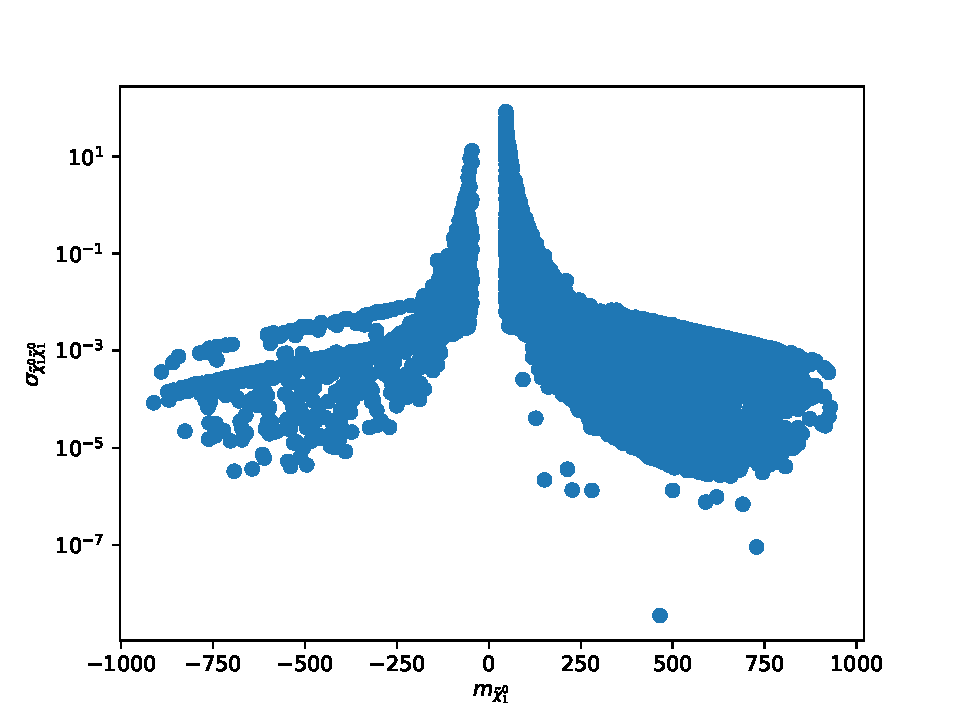
\includegraphics[scale=0.7]{figures/dataset/masses.pdf}
    \caption{The values of the cross sections $\sigma_{\tilde{\chi}_1^0 \tilde{\chi}_1^0}$ are shown projected onto the axis of masses $m_{\tilde{\chi}_1^0}$. The data is taken from the training data.
    }\label{fig:dataset_masses}
\end{figure}


\begin{figure}[h!]
    \centering
    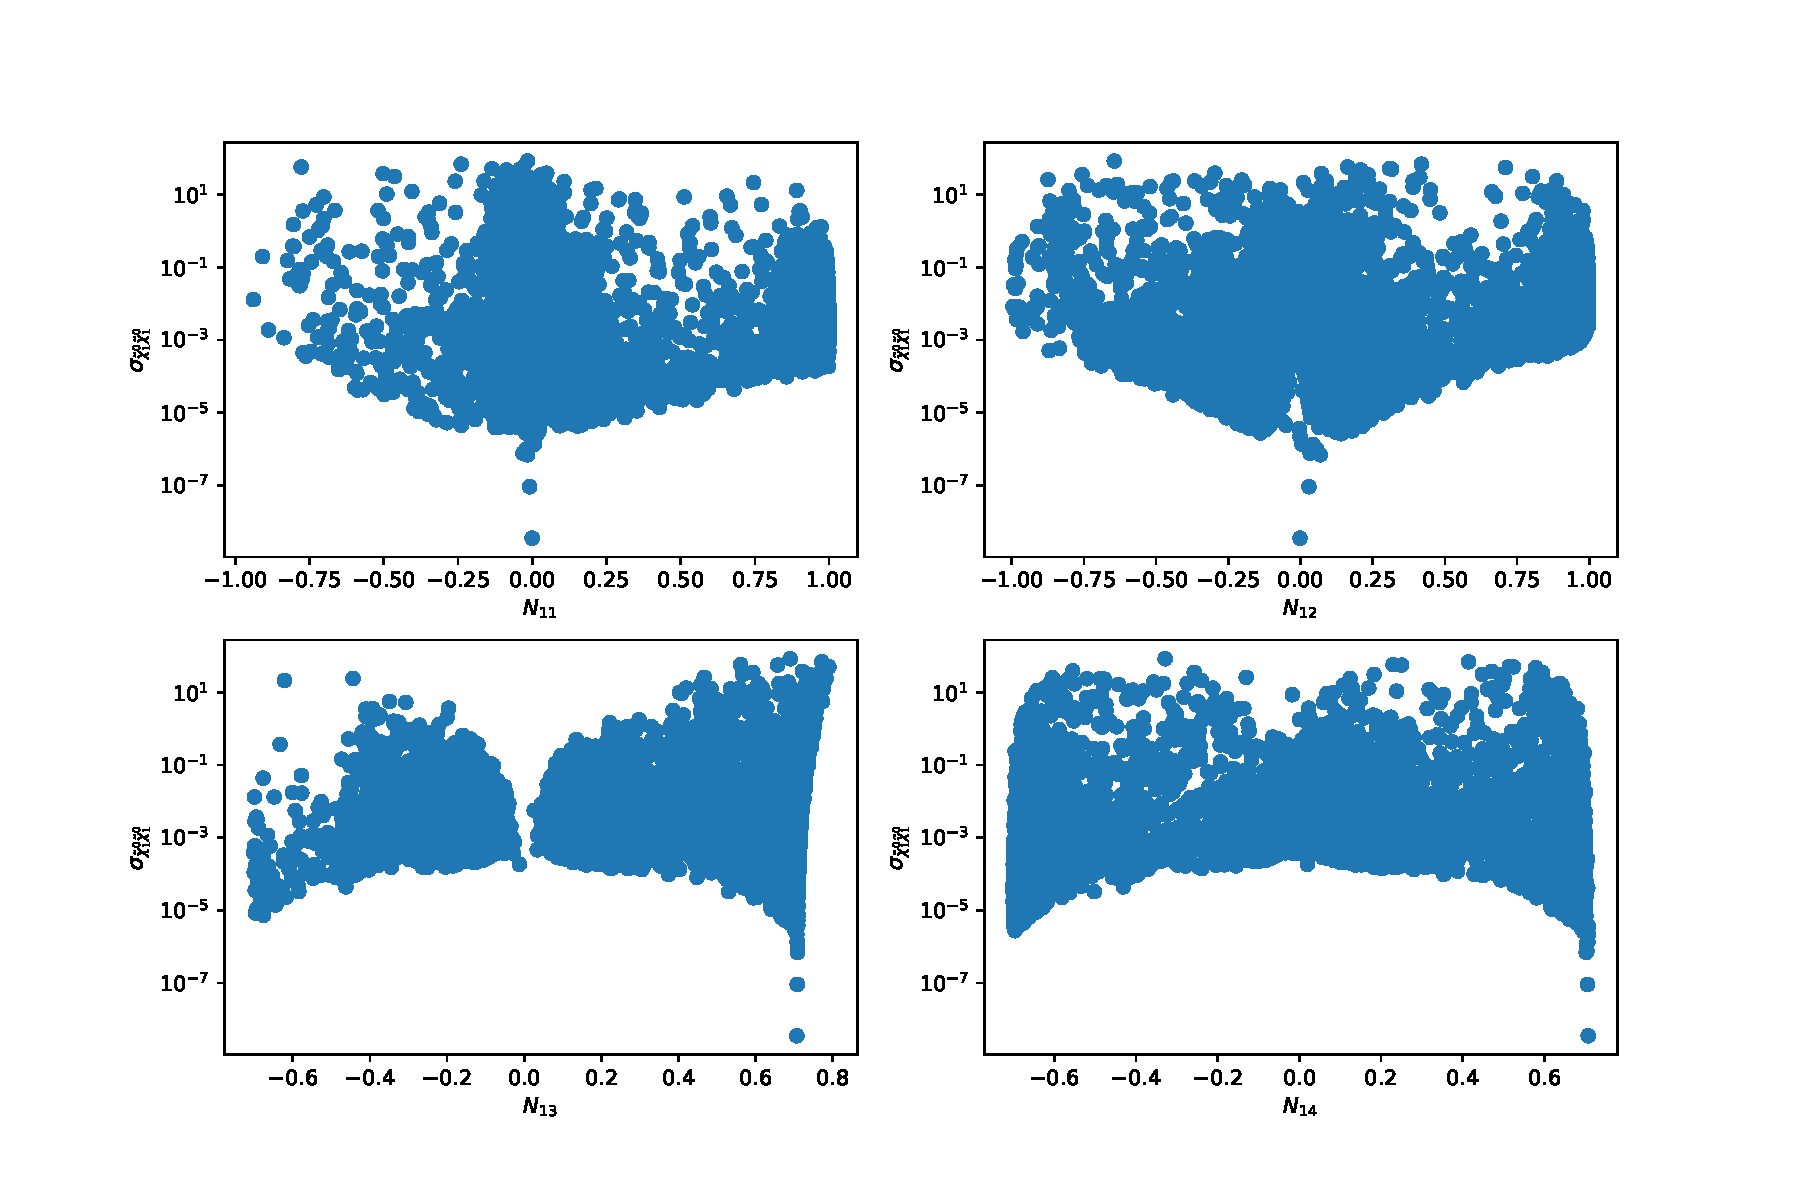
\includegraphics[scale=0.5]{figures/dataset/mixing_angles.pdf}
    \caption{The values of the cross sections $\sigma_{\tilde{\chi}_1^0 \tilde{\chi}_1^0}$ are shown projected onto the axes of mixing angles $N_{1j}$ for $j = 1, 2, 3, 4$. The data is taken from the training data.
    }\label{fig:dataset_mixing_angles}
\end{figure}


\subsection{Data Transformations}\label{sec:data_transform}
We shall briefly discuss how the training data is transformed before training.
The targets in the dataset of NLO cross sections can span several orders of magnitude. For practical training of BNNs, this would require
model parameters that also span several orders of magnitude. The result will usually be overflow and thus unsucessful training of the models.
Therefore, we have chosen to map the targets using the base-10 logarithm, i.e. $y \mapsto \log_{10}(y)$. More generally, we could choose any base-$a$ logarithm. A practical consideration here is that once the model is trained, any prediction it produces must be transformed back using
the inverse mapping to produce a cross section. As we increase the value of $a$, the precision the model's prediction decreases. Thus a small error in log-space 
can result in a large error in what we may refer to as the target space, the larger the value of $a$ is. 
We will explore the performance both in log space using the transformed data and in target space by applying the inverse mapping to the predictions.


\begin{comment}
    \subsubsection{Error Propagation}
As we discussed in section \ref{sec:data_transform}, we perform the mapping $y \mapsto \log_{10}(y)$ on the targets in the training data. Thus our BNN models will train on targets in log space and its predictions will reside in the same space. Let us denote its predictions as $\hat{y}$ which we treat as a stochastic variable since it produces a predictive distribution given an input $x$. Suppose $\hat{y}_\text{mean}$ is the sample mean of its predictions and $\sigma_{\hat{y}}^2$ is the sample variance. Let us denote $\hat{f} = {10}^{\hat{y}}$ as its prediction transformed back to target space. The differential of $\hat{f}$ is
\begin{equation}
    \dd \hat{f} = \dd \hat{y} \ 10^{\hat{y}} \ln(10).
\end{equation}
Treating $\dd \hat{y} \to \sigma_{\hat{y}}$ and $\dd \hat{f} \to \sigma_{\hat{f}}$ we can approximate the error propagated from log space onto target space as
\begin{equation}
    \sigma_{\hat{f}} \approx \sigma_{\hat{y}} \ 10^{\hat{y}} \ln(10),
\end{equation}
where $\hat{y}$ is understood as the sample mean of the 
\end{comment}

\begin{comment}
    A final aspect we mention is that only $a$ on the form $a = 2^b$ for an integer $b \geq 0$ will yield transformed data that can be represented exactly on a computer. Any other transformation automatically introduces a truncation or rounding error once the transformation is performed which introduces a small systematic error in the training data \textit{before} even training has begun. 
\end{comment}

\subsection{Data Splitting}
\textit{Data splitting} is a common strategy in machine learning to avoid biased model selection and obtain reliable estimates of the performance of the trained models.
The conventional way is to split the dataset $\mathcal{D}$ into three subsets: 
\begin{enumerate}
    \item A training set $\mathcal{D}_\text{train}$. This dataset usually contain the largest chunk of the dataset and is used to train the models.
    \item A validation set $\mathcal{D}_\text{val}$. This dataset is typically the smallest of the bunch and is sometimes used in classical machine learning problems to perform cross-validation or similar methods. The results measured here are typically used to select hyperparameters of the model.
    \item A test set $\mathcal{D}_\text{test}$. This partition is slightly larger than the validation set and is used as an out-of-sample check to measure the performance of a model. 
\end{enumerate}
We have selected to use a division of 80\% training data, 5\% validation data and 15\% test data. In practice though, the notion of a validation set does not lend itself as easily to Bayesian ML tasks and we may in practice therefore use both the validation and test data as the test set.

\section{Methodology}
In this section, we shall explain the methodology used to train and test the BNNs explored in this thesis. We will explain the implementations, selection of models and hyperparameters and performance metrics used.

\subsection{Implementation}
We have utilized the Python libraries {\tt TensorFlow 2.7.0} and {\tt TensorFlow-Probability 0.15.0} to implement the BNNs. 
The implementation itself is available at \url{LEGG TIL URL HER}. Unfortunately, BNNs trained with HMC or NUTS has not been of interest for majority of the deep learning community. The main focus has been with use of surrogate distributions to develop algorithms that when employed using GPUs spend roughly the same amount of time per epoch as training of classical neural networks. As a result no implementations of BNNs for these kind of samplers have been implemented directly into the either framework. Luckily, {\tt TensorFlow-Probability} provide general purpose implementations of the samplers we have discussed hithertho 
which only requires us to define the \textit{unnormalized negative log-target density} (which is the negative potential function -$\mathcal{L}$) to utilize the them. 
Consequentially, we created our own class that facilitates the usual kind of conveniences shipped with {\tt TensorFlow} such as the ability to automatically save, load or print the model architecture to screen, to name as few. The class and its functionality is well-documented and made with the intention to be reused, expanded and modified. 

Both {\tt TensorFlow} and {\tt TensorFlow-Probability} handle execution on NVIDIA GPUs automatically with minimal effort on the user side, which we have utilized to generate our results. We will also provide measurements that indicate the expected speedup gained from using a GPU instead of a CPU for training of BNNs. Some of the results are also generated using the built-in GPU on an M1 Apple Silicon system-on-chip (SoC), since a port that supports execution on this device is available. In any case where computational performance is measured, we will make it crystal clear on what hardware the calculations are performed.
 

\subsection{Selection of Models and Hyperparameters}
In order to better understand the behaviour of BNNs, we have chosen to train a set of models whose details are listed in table \ref{tab:deep_models}. Each model consists of 1000 sampled neural networks. Each model is trained with $\tanh(x)$ as the activation function on the hidden layers, while the output layer uses an identity activation. We will refer this table whenever a model or a set of models selected from it is used. Otherwise, we will state the model architecture used and its hyperparameters explicitly. 
\begin{table}[h!]
    \centering
    \caption{
        The table shows the models used in this section. For each model, 1000 sampled networks were sampled to collectively represent each BNN model. We used 2500 warm-up steps (20\% burn-in and 80\% adaptation). We skipped 10 samples for each sampled network. We performed 1000 pretraining epochs with a batch size of 32 using the ADAM optimizer. The kernel used for each model was the NUTS kernel with a maximum of $L = 4096$ Leapfrog steps.
        The number of nodes per layer is shown in the ``Layers'' column.
        For each hidden layer, we used $\tanh(x)$ as the activation function. The final layer used an identity activation.
    }
\begin{tabular}{c@{\hspace{1cm}}c@{\hspace{1cm}} c}
\hline
      Model number & Layers & Number of parameters \\
\hline
    1 & 5-50-1 & 351\\
    2 & 5-50-50-1 & 2901\\
    3 & 5-50-50-50-1 & 5451\\
    4 & 5-50-50-50-50-1 & 8001\\
    5 & 5-50-50-50-50-50-1 & 10551\\
\hline
\end{tabular}
\label{tab:deep_models}
\end{table}


\subsection{Performance Metrics}\label{sec:perf_metrics}
In this section, we will discuss the performance metrics used to benchmark and measure the performance of the models trained in this thesis.
Due to the inherent probabilistic nature of the models trained, any output the model produces will be a distribution from which we can calculate
a sample mean and variance. 
We will introduce a metric to measure the performance of the mean predictions of the BNNs called coefficient of determination and a metric to assess the BNNs ability to yield reliable uncertainties in its predictions called standardized residuals.

\subsubsection{Coefficent of Determination}
The \textit{coefficent of determination}, or the $R^2$-\textit{score}, is used to assess the quality of the predictions of a model in supervised regression tasks. For a dataset $\mathcal{D} = \{(x^{(i)}, y^{(i)})\}_{i=1}^N$, it is given by
\begin{equation}\label{eq:r2_score}
    R^2 = 1 - \frac{\sum_{i=1}^N (y^{(i)} - \hat{y}^{(i)})^2}{\sum_{i=1}^N (y^{(i)} - \bar{y})^2},
\end{equation}
where $y^{(i)}$ denotes the target of an input $x^{(i)}$ and $\hat{y}^{(i)}$ denotes the model prediction and $\bar{y}$ denotes the sample mean of the targets
\begin{equation}
    \bar{y} = \frac{1}{N}\sum_{i=1}^N y^{(i)}.
\end{equation}
The $R^2$-score lies in the range $R^2 \in (-\infty, 1]$ where the larger the value, the better the model predicts. The score is interpreted as the proportion of the variance in the targets that can be predicted from the inputs. The reason we select this metric is that it provides a more reliable interpretation of the prediction quality of our models than other metrics such as mean squared error (MSE), root mean squared error (RMSE) and the mean absolute error (MAE) which can only be used to compare the predictions of models relative to each other \cite{r2_score}. Their values all lie in the range of $[0, \infty)$ where a perfect prediction would yield zero. The lack of an upper-bound on these alternative metrics make them difficult to interpret in a vacuum, a weakness the $R^2$-score does not suffer from. If $R^2 < 0$, the model performs poorly, while of $R^2 \in [0, 1]$, the model explains the variation in the data with $R^2 = 0$ meaning the model cannot explain any of the variance in the targets around their sample mean. A score of $R^2 = 1$ means a perfect prediction.

Note that when we use BNNs to compute the $R^2$-score, we will replace $\hat{y}^{(i)}$ in eq.~\eqref{eq:r2_score} with the sample mean of the predictive distribution computed by the BNNs. 

\subsubsection{Standardized Residuals}
\textit{Standardized residuals} is a transformation of a model prediction given an input feature $x^*$ and a target $y^*$. The mapping is defined as
\begin{equation}\label{eq:standardized_residuals}
    z(x^*) = \frac{y^* - \hat{y}_\text{mean}(x^*)}{\hat{\sigma}(x^*)},
\end{equation}
where $\hat{\sigma}(x^*)$ is the square-root of the sample variance of the model predicitions and $\hat{y}_\text{mean}(x^*)$ is the sample mean of the predictions and. The mapping in eq~\eqref{eq:standardized_residuals} resembles the mapping of a random variable $x \sim \mathcal{N}(\mu, \sigma^2)$ onto the standard Normal distribution $z \sim \mathcal{N}(0, 1)$.


As we discussed in chapter \ref{chap:bayesian_ml}, the fundamental assumption made is that any target $y$ can be decomposed as
\begin{equation}
    y = f(x) + \delta,
\end{equation}
for some true function $f(x)$ and a random noise $\delta \sim \mathcal{N}(0, 1)$, i.e it is distributed according to a standard Normal distribution. But the noise in the data produced by \texttt{Prospino} is neglible, which means that $y \approx f(x)$. The regression error obtained through the sample variance of the model predictions must therefore be dominated by the variance of the predictive distribution computed by the model itself. Let $\sigma_z^2$ denote the variance of the distribution of the standardized residual. If $\sigma_z > 1$, the model will be considered overconfident in its predictions since the sample variance of the model's predictions are smaller than the variance of the targets around the mean prediction. On the other hand, if $\sigma_z \leq 1$, we consider the model to yield reliable uncertainty estimates. In this case, the model is not considered to be ``underconfident'' but rather ``conservative''.



\section{Results and Discussion}\label{sec:results}
In this section we present the results from various numerical experiments and discuss their implications. We start off with measurement of computational performance with a focus on training time, prediction time and loading times. We then investigate the posterior distribution projected onto a 2-dimensional planes of the BNN weights to investigate their property with a focus on whether typical approximations made in the literature provides a sufficient representation of the exact posterior distribution. Following this, we present the effect of various hyperparameters pertaining to the training of BNNs, including the performance achieved when using HMC and NUTS. Finally, we explore the predictive distributions of various trained BNNs.

\subsection{Computational Performance}
In this section we will explore the computational performance of BNN models, both on modern CPUs and GPUs. We shall measure the training time which with the way we perform Bayesian inference of the BNN parameters most appropriately translates to the time used per generated sample with HMC and NUTS. Another measurement of great interest is the time a trained BNN model used to compute predictions as this will be their central usage once trained. But because we must store the full BNN model on disk, the loading times play an important role as well. We shall therefore measure both the execution time of predictions and loading times separately.
We will perform wall clock measurements using {\tt time.perf\_counter} provided by the {\tt time} module of the standard library shipped with Python 3. It yields a measurement in fractional seconds of the clock with the highest available resolution on the system.

\subsubsection{CPU v. GPU Performance}
In this thesis we are primarily concerned with creation of an optimized alternative to direct calculations of cross sections.
An important consideration is at which available commercially available hardware platform the most speedup can be achieved. In this section
we pin the performance of available CPU and GPU hardware against each other. First note that {\tt TensorFlow} and its framework supports OpenMP-type parallelization on the CPU, that is, parallelization where a single node consisting of several cores, or in the case case of a CPU that supports hyperthreading, a set of virtual threads exceeeding the number of physical cores that evenly divide the workload within the compute node, using a shared memory parallelization strategy similar to what a GPU does. Unfortunately, multi-device parallelization either on the CPU or the GPU lacks support, particularly in the case of non-synchronous execution. Thus in this section we will only compare performance of the single-node performance that is achievable with either a CPU or GPU. We will thus contrast the performance achieved by a single CPU node with several (virtual) cores available to the performence obtained by employing the most taxing workload on a GPU.
In figure \ref{fig:relative_performance}, we demonstrate the significant speedup that can be achieved
with GPU accelerated sampling when using {\tt TensorFlow-Probability} and its implementation of samplers. Here we have used HMC and a fixed $L = 512$ Leapfrog steps with XLA (Accelerated Linear Algebra) compilation enabled on the GPU. This is a highly optimized linear algebra execution engine that can significantly speed up code written with {\tt TensorFlow} run on the GPU \cite{xla}. The time measurements per sample was in the order of magnitude of seconds for the most complex models
tested. An important aspect for practical utilization of BNNs will be ease of training and accelerated sampling with NUTS or HMC, which is automatically achieved if the system can detect an NVIDIA GPU. Moreover, the full training time can be estimated by a few preliminary runs where execution time per sample is measured. This analysis is slightly more difficult when using NUTS. One can however set a maximum tree depth $J$ which translates to a maximum of $L = 2^J$ Leapfrog steps when using the implementation in {\tt Tensorflow-Probability}. As we argued in chapter \ref{chap:no_u_turn_sampler}, the additional computational cost added by NUTS per Leapfrog step is neglible given a sufficiently complex model and/or large dataset, so measurement of the time per sample used by HMC with a fixed $L$ provides a sensible estimate of the maximal time used by NUTS per sample if the maximum tree depth is set to the corresponding number of Leapfrog steps used.
Thus one can simply perform the measurements using the implementation of HMC and estimate an upper-bound on the computational time.

\begin{figure}[h!]
    \centering
    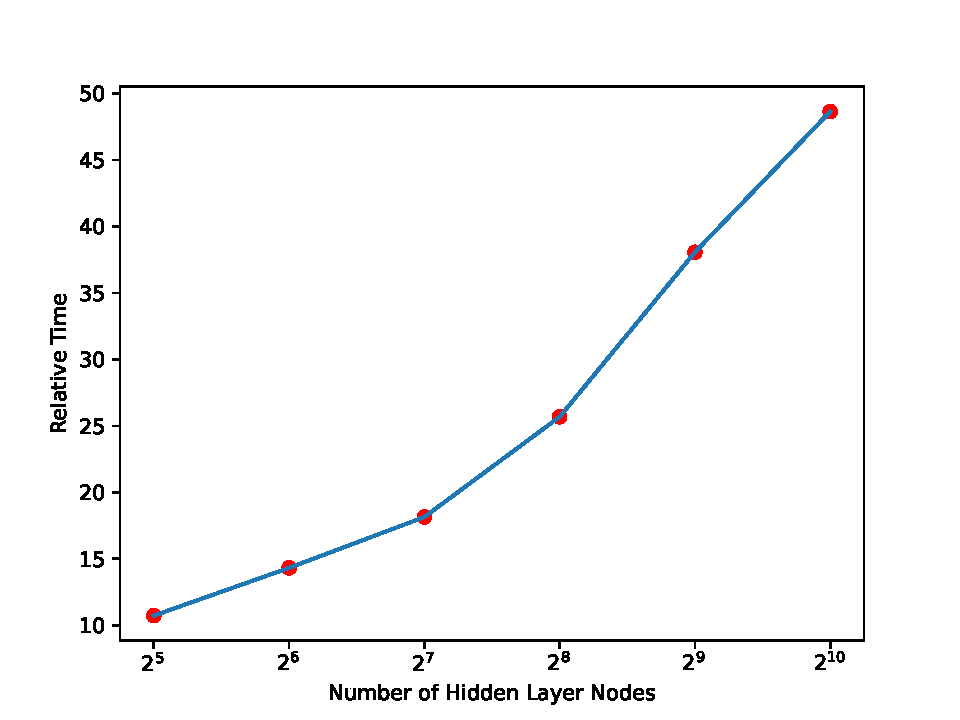
\includegraphics[scale=0.7]{figures/cpu_vs_gpu/cpu_vs_gpu_performance.pdf}
    \caption{The figure shows the relative measured execution time used per sample using $L = 512$ Leapfrog steps,
    as a function of number of parameters. The CPU measurements are done using an 8-core M1 CPU (Apple Silicon). The GPU measurements
    are made with an NVIDIA Tesla P100 GPU.
    }
    \label{fig:relative_performance}
\end{figure}

\subsubsection{Prediction Time}
As we discussed in the introduction, the execution time's order of magnitude when using {\tt Prospino} is in the order of hours. 
If BNNs are to serve as a viable alternative to these calculations, it must at least significantly reduce the time it takes to compute predictions. In figure \ref{fig:prediction_time}, we 
show the average execution time to compute predictions using all models in table~\ref{tab:deep_models}.
For each model, we randomly generated input points of correct dimension and computed predictions for up to 4096 input points simultaneously.
The execution times appear proportional to the number of input points provided for each model, which perhaps is not all that surprising. We can crudely infer by inspection that increasing the order of magnitude by one does the same for the execution time. Still, the order of magnitude for a single input point is at the order of a millisecond which is a significant speedup over {\tt Prospino} calculations. Both the sample mean of the predictions and the sample error is computed during the measurement. The measurements were performed on an M1 Apple Silicon CPU using {\tt perf\_counter} from the module {\tt time} provided by the standard library of Python.

The performance degradation that the computations in figure \ref{fig:prediction_time} suffers is inherently due to the limited vectorization capability of the CPU's computing units when performing matrix multiplications in the forward pass of the individual neural network models. The computation itself is performed with all 1000 sampled networks simultaneously, and so one might hypothesize that more specialized computing units may be able to handle several input points while applying all sampled networks at the same time. As it turns out, GPUs are excel at executing matrix multiplication and even more fortunate, {\tt TensorFlow} has added support for the built-in GPU on Apple Silicon system-on-chips. In figure \ref{fig:prediction_time_gpu} we can see the execution times achieved using the GPU to perform the same computations as before. In this case the order magnitude remains more or less the same in all the tests. Thus, computing predictions on several points can benefit greatly if the execution is employed on a GPU. Note, however, that the measured execution time of ``model 1'' is slightly slower than for more points which likely is due to the overhead introduced by using the GPU for such a simple model. Care must thus be taken when considering what type of hardware the computations should be performed with.

\begin{figure}[h!]
    \centering
    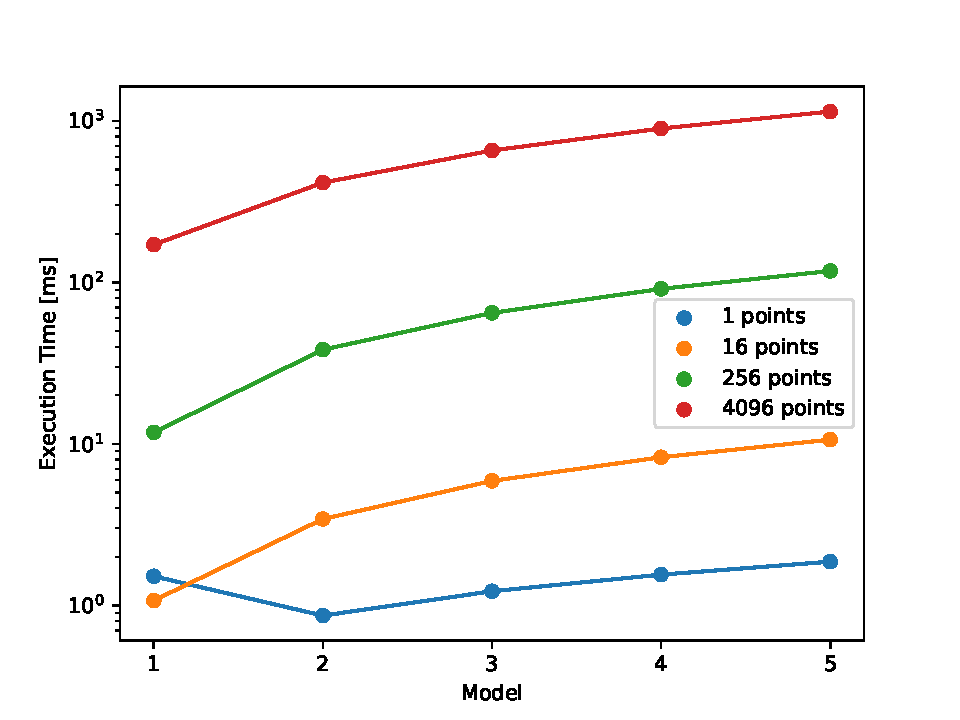
\includegraphics[scale=0.7]{figures/prediction_time/prediction_time.pdf}
    \caption{The figure shows the average prediction time to compute a prediction given a single input $x$ using the models in table \ref{tab:deep_models}. The average time used is measured in ms and is averaged over 1000 randomly sampled points. The measured time includes computation of the sample mean and sample error.
    }
    \label{fig:prediction_time}
\end{figure}

\begin{figure}[h!]
    \centering
    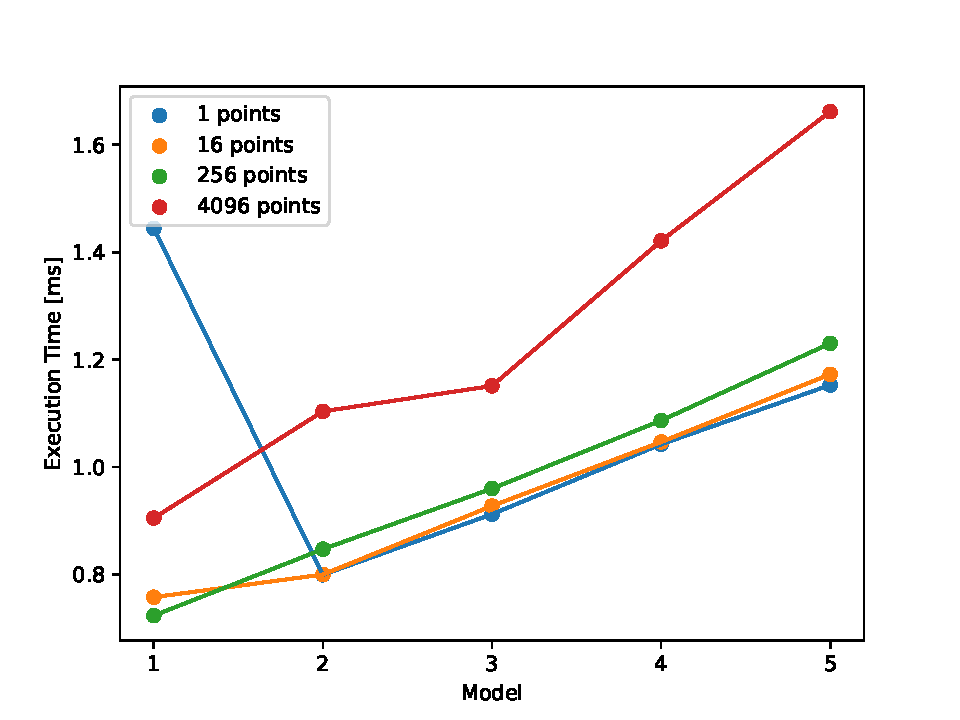
\includegraphics[scale=0.7]{figures/prediction_time/prediction_time_gpu.pdf}
    \caption{The figure shows the average prediction time using the built-in GPU on an M1 Apple Silicon system-on-chip to compute a prediction given a single input $x$ using the models in table \ref{tab:deep_models}. The average time used is measured in ms and is averaged over 1000 randomly sampled points. The measured time includes computation of the sample mean and sample error. 
    }
    \label{fig:prediction_time_gpu}
\end{figure}

\subsubsection{Loading Times}
Even if we have demonstrated a substantial speedup for predictions using BNNs, we have thus far ignored the fact that empirical distribution representing the weights of the BNN is stored on disk which typically means an solid state drive (SSD) with modern computing hardware. The memory bandwidth between the SSD and the faster forms of memory such as RAM, cache and registers becomes a potential bottleneck for performance. Although cache and registers introduce fast memory transfer of stored data to the computing units of the CPU, they typically boast a fairly limited capacity. Thus loading in the entire BNN model might not be viable and we may observe that once we need to models with a large number of parameters, the loading times dominate the computational cost involved with computing predictions. This added computional cost stems from the transfer of data back and forth between the RAM, and the cache and registers. An additional problem is that if the BNN model is simply used for a single prediction at a time, it might simply be loaded a single time before it is dumped from working memory all together. In this case, the initial load may dominate the computational cost all together. 

In figure \ref{fig:loading_times} we show the resulted loading times measured using an M1 Apple Silicon system-on-chip and {\tt time.perf\_counter} from Python. The memory allocated to the BNN models were deallocated manually using the {\tt del} operator provided by Python to ensure that each load of the model of the model was from the SSD. The models loaded in are the ones listed in table \ref{tab:deep_models}. Given the order of magnitude of the loading times displayed in the figure is approximately the same order of magnitude as the execution time, we have demonstrated that BNNs can provide a serious substitute for {\tt Prospino} calculations from a purely computational perspective. It remains to be seen if the predictions themselves are reliable enough for this substitution to be adopted, which we will explore in later sections.

\begin{figure}[h!]
    \centering
    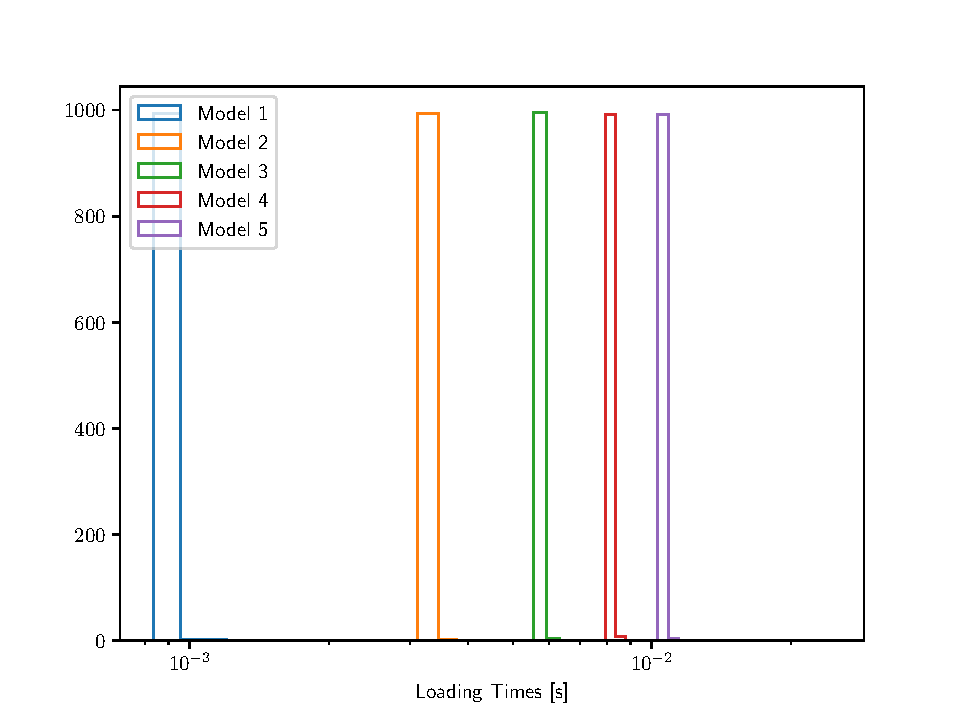
\includegraphics[scale=0.7]{figures/computational_cost/loading_times.pdf}
    \caption{
        The figure shows the histograms of measured loading times in seconds using the models in table \ref{tab:deep_models}. The measurements were performed using {\tt time.perf\_counter} from Python using an M1 Apple Silicon system-on-chip. The time measurements consist of 1000 measurements for each model.
    }
    \label{fig:loading_times}
\end{figure}



\subsection{Posterior Distribution of Weights}
An important problem to consider is if we can even justify the use of Monte Carlo samplers to sample from the exact posterior instead of using the approximation employed by variational inference with a parameterized surrogate posterior which is the most ubiquitous method of training BNNs in the literature. The surrogate distribution is usually a factorized normal distribution of the form
\begin{equation}\label{eq:surrogate_dist}
    q \propto \prod_{i, j, \ell} \mathcal{N}(\mu_{ij}^\ell, (\sigma_{ij}^\ell)^2) \mathcal{N}(\mu_{j}^\ell, (\sigma_{j}^\ell)^2),
\end{equation}
meaning for each parameter in the model, we assume its posterior distribution can be written as an independent Gaussian distribution with a mean $\mu_{jk}^\ell$ and a standard deviation $\sigma_{ij}^\ell$ for the kernels, and $\mu_j^\ell$ and $\sigma_j^\ell$ for the biases. The method sports some fairly obvious advantages like the fact that one can perform \textit{online training}, i.e. continue training once new data becomes available starting from an earlier \textit{checkpoint} by using $q$ obtained during earlier training as the prior. The way we have trained BNNs in this thesis does not permit this form of training because we cannot formulate a prior based on the empirical distribution we have sampled. Thus we cannot use the weights of the model that we have already sampled to continue training. We must start over entirely and discard the empirical distribution we obtained with the prior dataset. 

It has been widely discussed that BNN posteriors are typically found to be multi-modal \cite{google_bnn_posteriors}. We demonstrate this observation in figure \ref{fig:posterior_kernels}.
We can observe that the projection onto the planes shown there indicate that the posterior distribution indeed is multimodal
and unlikely to be approximated well with a parameterized surrogate distribution like the one in eq.~\eqref{eq:surrogate_dist}.

\begin{figure}[h!]
    \centering
    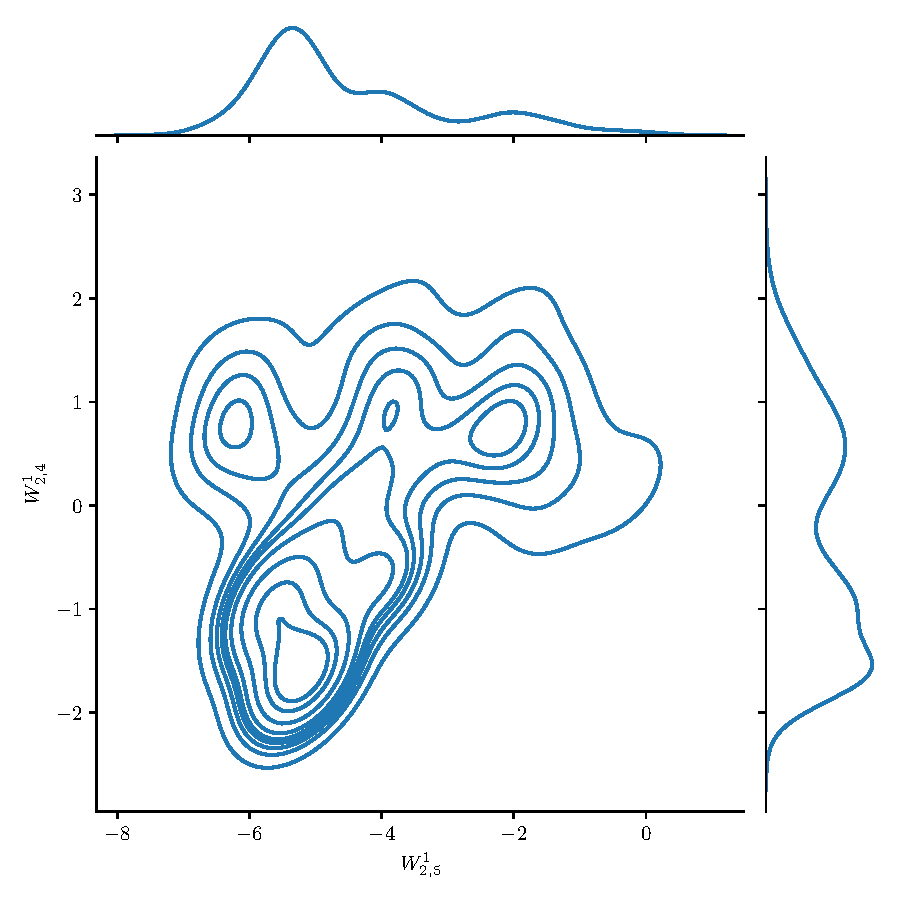
\includegraphics[scale=0.7]{figures/posterior_distribution/posterior_weights1.pdf}
    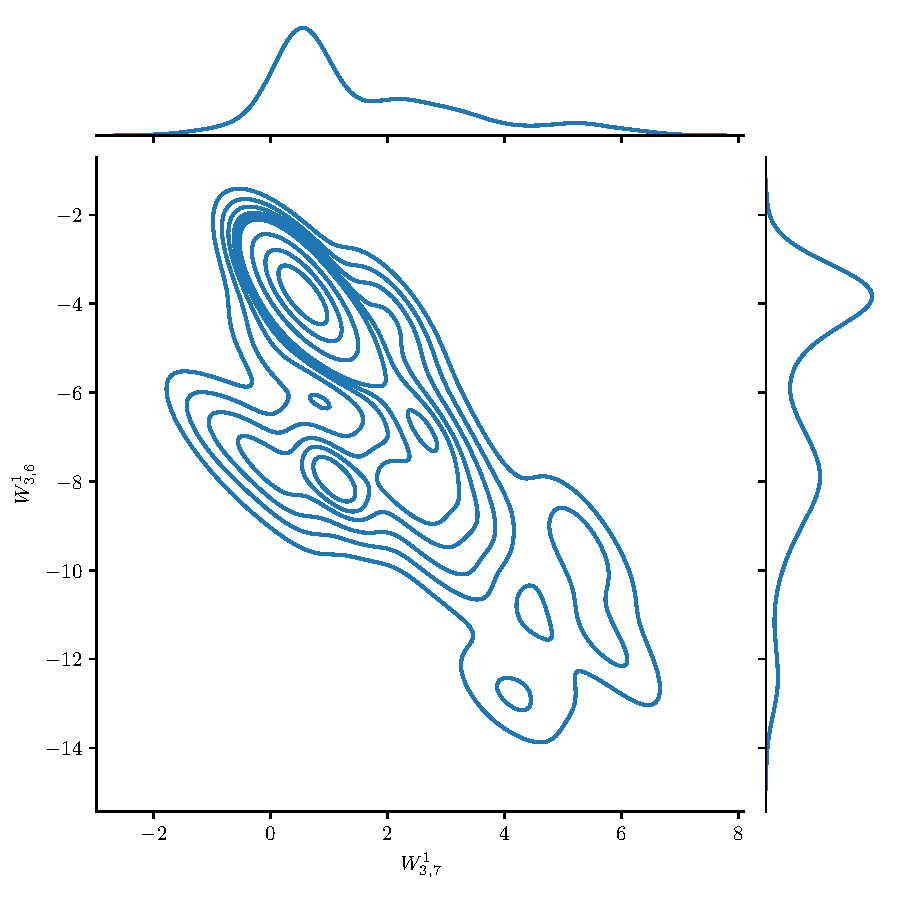
\includegraphics[scale=0.7]{figures/posterior_distribution/posterior_weights2.pdf}
    \caption{The figure shows the projection of the empirical distribution onto the planes spanned by $(W_{2,4}^1, W_{2,5}^1)$ on the left and onto the plane spanned by $(W_{3,7}^1, W_{3, 6}^1)$ on the right, using the samples from model 3 in table \ref{tab:deep_models}. The distributions are approximated using kernel density estimation. 
    }
    \label{fig:posterior_kernels}
\end{figure}


\subsection{Benchmarks of Hyperparameters}\label{subsec:benchmarks}
\begin{figure}[h!]
    \centering
    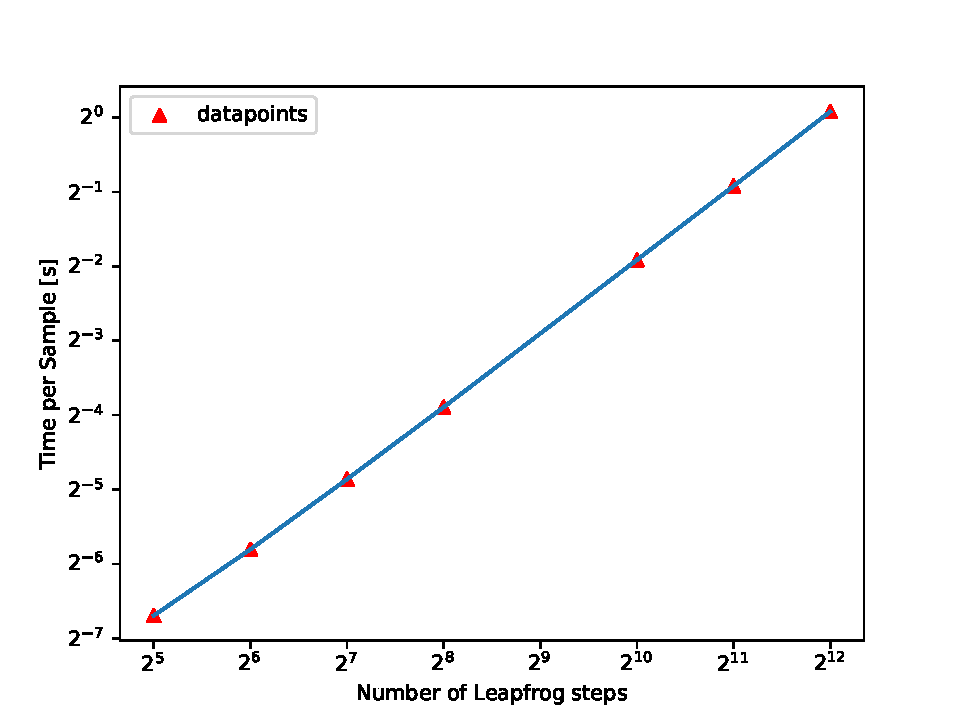
\includegraphics[scale=0.7]{figures/computational_cost/time_vs_leapfrogsteps_hmc.pdf}
    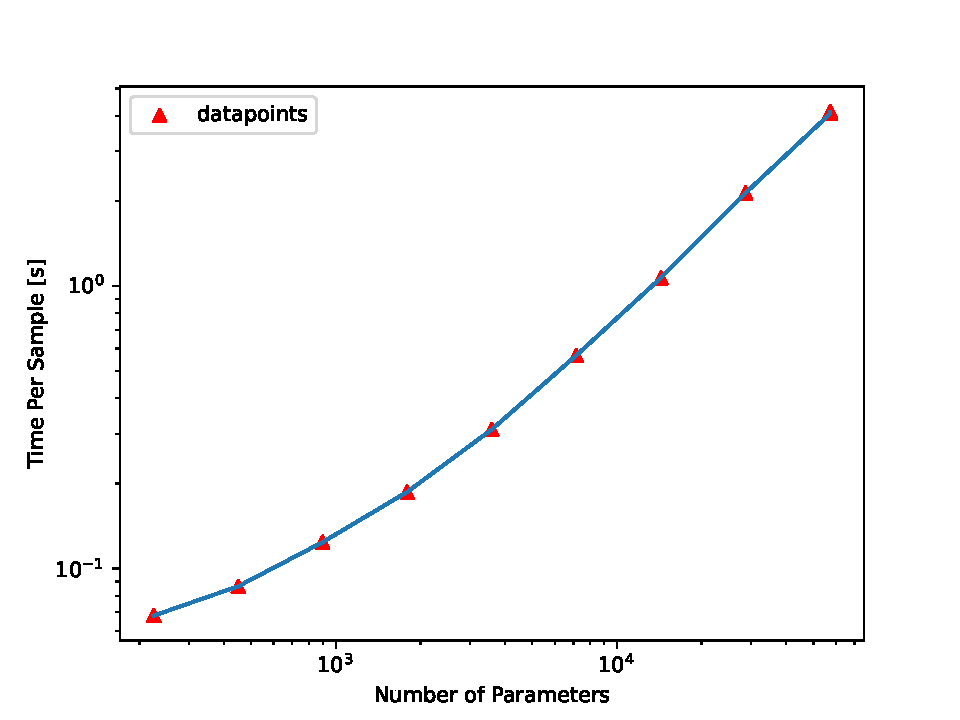
\includegraphics[scale=0.7]{figures/computational_cost/time_vs_params.pdf}
    \caption{The figure at the top shows the measured time in seconds per sample using HMC as a function of Leapfrog steps $L$ using a model with
    561 parameters. The figure at the bottom shows the time in seconds per sample with the same sampler with a fixed number of Leapfrog steps $L = 512$ as a function of number of parameters in the BNN model.
    }
    \label{fig:time_vs_leapfrogsteps}
\end{figure}

\subsubsection{The Effect of Number of Warm-up Steps}
As we discussed in section \ref{sec:practical_bnn}, we must set a predetermined number of warm-up steps, i.e. number of burn-in steps and number of adaptation steps when using {\tt TensorFlow Probability}'s samplers.
Conventional wisdom would have us believe that increasing the number of burn-in steps increases the probability that the Markov chain has converged
to the stationary distribution of the posterior. Moreover, the literature has shown that NUTS performs at least as good as or better than HMC with an equivalent number of maximum Leapfrog steps or more as the results in \cite{nuts} demonstrated. In our case we have split the number of warm-up steps to 20\% burn-in steps and 80\% adaptation steps, respectively. This is a heuristic recommended by the {\tt TensorFlow Probability} developers.

To investigate the effect of the number of warm-up steps, we employed a model with a 5-20-20-1 architechture using $\tanh(x)$ as the activation function on the hidden layers. We fixed the number of pretraining epochs to 2500 with a batch size of 32 using the ADAM optimizer.
We then trained several models using various number of warm-up steps with both HMC and NUTS. When trained with HMC, we fixed the number of Leapfrog steps to $L = 512$. When trained with NUTS, we set a maximum tree depth of $12$ corresponding to a maximum of $L = 4096$ Leapfrog steps.
In figure \ref{fig:r2_score_vs_burn_in_steps} we show the achived $R^2$-scores of the different configurations both in log space and target space as function of the number of warm-up steps used. In log space, the models consistently achieve scores $R^2 \approx 1$ which suggest they on average correctly predict the targets in the test data. Transforming the predictions and targets back to target space, however, lead to som fairly poor results as we increase the number of warm-up steps with HMC outperforming the models trained with NUTS in all but one case. We removed the point at 32 warm-up steps for the NUTS sampler as it achieved a poor score of $R^2 = -1306$ in this case. It is difficult to explain this discrepancy as the $R^2$-score in log space is good. But the general observation to note here is that the performance of the models degrade once we transform back to target space which is expected as we discussed in section \ref{sec:data_transform} on the effect of the data transformations. At least we now have an empirical confirmation that suggests that reducing the base of the logarithm used to transformm the data should be investigated further.

In figure \ref{fig:standardized_residuals_vs_burn_in_steps} we display the standardized residuals in log space for both samplers over all trained configurations. 
The standardized residuals demonstrate that the claims discussed in the beginning of this section may not be general enough to apply to BNNs as the models trained with HMC performs better almost regardless of how many warm-up steps that are performed. When using NUTS, the performance of the model trained with a substantial amount of warm-up steps appear to degrade as opposed to improve consistent with their $R^2$-scores. The standardized residual of HMC lies consistently inside the Normal distribution for the bulk of the distribution albeit with longer tails, while the NUTS sampler produced rather few models that achieve the same. These results, then, actually indicate that we may be better off running the training procedure of BNNs with a fixed $L$, only adapting the step size. Even better, we may get by with a fairly small number of warm-up steps and a fairly small $L$. But the claim that NUTS performs at least as well as HMC with an equivalent number of Leapfrog steps begs the question, then, how many Leapfrog steps did NUTS use on average? In figure \ref{fig:avg_leapfrog_steps_vs_burn_in}, we show the average number of Leapfrog steps the NUTS sampler used during the generation of the Markov chain as a function of number of warm-up steps. Clearly, NUTS used more Leapfrog steps on average than $L = 512$, except in a single case. The NUTS sampler introduces the need for a slightly more complicated analysis than a one-to-one comparison like this though. Recall from chapter \ref{chap:no_u_turn_sampler}, that the NUTS sampler generates samples by running HMC forwards and backwards in time at random until a stopping condition is met. At this point the sampler selects one of the acceptable states that does not violate detailed balance at random. Thus the selected position (model parameter) may lie close to the initial position while HMC automatically selects the final position of the simulation. Thus for the same number of Leapfrog steps, we should expect HMC to generate larger jumps in parameter space when using the same step size. 

\begin{comment}
\begin{table}[h!]
    \centering
    \caption{
        The table shows the computed $R^2$-scores in both log space and target space for an increasing number of warm-up steps (20\% burn-in and 80\% adaptation) achieved with HMC and NUTS. The architecture of the BNN model used is 5-20-20-1 with $\tanh(x)$ used as the activation function in the hidden layers. We performed 2500 pretraning steps with a batch size of 32 using the ADAM optimizer. In total 1000 neural networks were sampled with 10 steps between each stored sample. When HMC was used, we ran with a fixed number of Leapfrog steps $L = 512$. When the NUTS sampler was used, we allowed for a maximum of $L = 4096$ Leapfrog steps (a maximum tree depth of $12$).
    }
\begin{tabular}{c@{\hspace{1cm}}c@{\hspace{1cm}}c@{\hspace{1cm}} c}
\hline
    Sampler & Warm-up steps & $R^2$ (Log space) & $R^2$ (Target space)\\
\hline
    HMC & 32 & 0.990 & 0.950 \\
    HMC & 128 & 0.992 & 0.950 \\
    HMC & 512 & 0.991 & 0.915 \\
    HMC & 2048 & 0.988 & 0.948\\
    HMC & 8192 & 0.990 & 0.877\\
    NUTS & 32 & 0.989 & -1306 \\
    NUTS & 128 & 0.991 & 0.917 \\
    NUTS & 512 & 0.991 & 0.931 \\
    NUTS & 2048 & 0.987 & 0.855 \\
    NUTS & 8192 & 0.987 & 0.855 \\
\hline
\end{tabular}
\label{tab:r2_burn_in}
\end{table}
\end{comment}

\begin{figure}[h!]
    \centering
    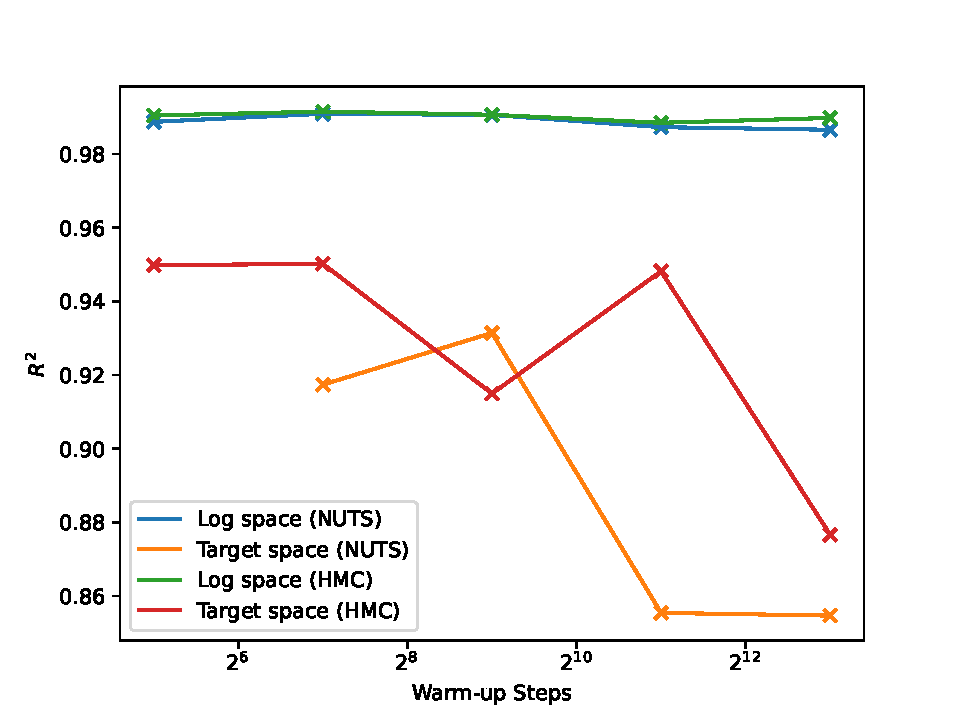
\includegraphics[scale=0.7]{figures/r2_scores/effect_of_burnin_r2_scores.pdf}
    \caption{
        The figure shows the computed $R^2$-scores in both log space and target space as a function number of warm-up steps (20\% burn-in and 80\% adaptation) achieved with HMC and NUTS. The architecture of the BNN model used is 5-20-20-1 with $\tanh(x)$ used as the activation function in the hidden layers. We performed 2500 pretraning steps with a batch size of 32 using the ADAM optimizer. In total 1000 neural networks were sampled with 10 steps between each stored sample. When HMC was used, we ran with a fixed number of Leapfrog steps $L = 512$. When the NUTS sampler was used, we allowed for a maximum of $L = 4096$ Leapfrog steps (a maximum tree depth of $12$).
    }
    \label{fig:r2_score_vs_burn_in_steps}
\end{figure}


\begin{figure}[h!]
    \centering
    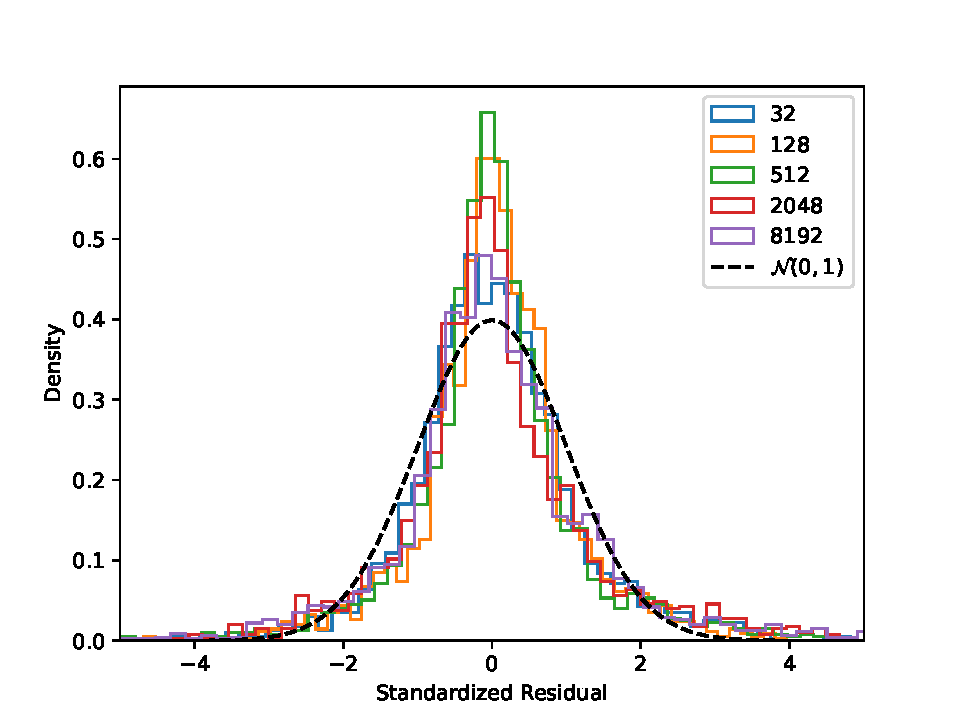
\includegraphics[scale=0.7]{figures/standardized_residuals/effect_of_burnin/standardized_residuals_hmc_vs_burn_in_steps.pdf}
    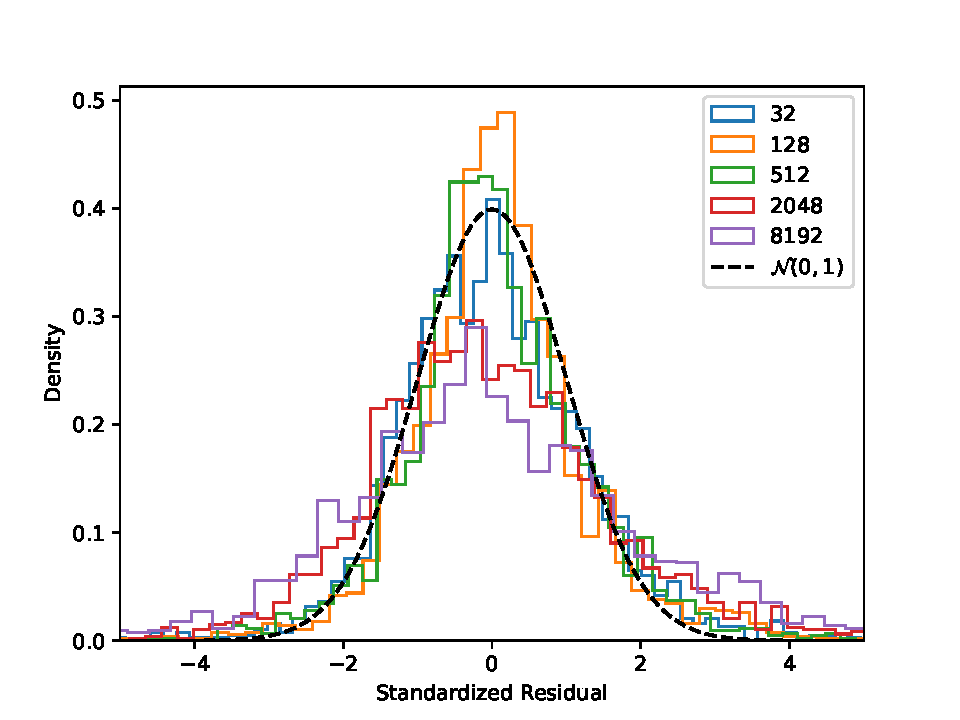
\includegraphics[scale=0.7]{figures/standardized_residuals/effect_of_burnin/standardized_residuals_nuts_vs_burn_in_steps.pdf}
    \caption{The figure shows the standardized residuals computed on the testset. The model architechture used is a model with layers 5-20-20-1 with $\tanh(x)$ as the hidden activation function. In the top figure, we have used the HMC sampler with a fixed number of Leapfrog steps $L = 512$. In the bottom figure, we have used the NUTS sampler with a maximum tree depth of $12$ corresponding to a maximum of $L = 2^{12} = 4096$ Leapfrog steps. The remaining important hyperparameters were 2500 pretraining epochs with a batch size of 32 using the ADAM optimizer. In total a 1000 neural networks were sampled in each case with a thinning-amount of 10 steps between each sample.
    }
    \label{fig:standardized_residuals_vs_burn_in_steps}
\end{figure}


\begin{figure}[h!]
    \centering
    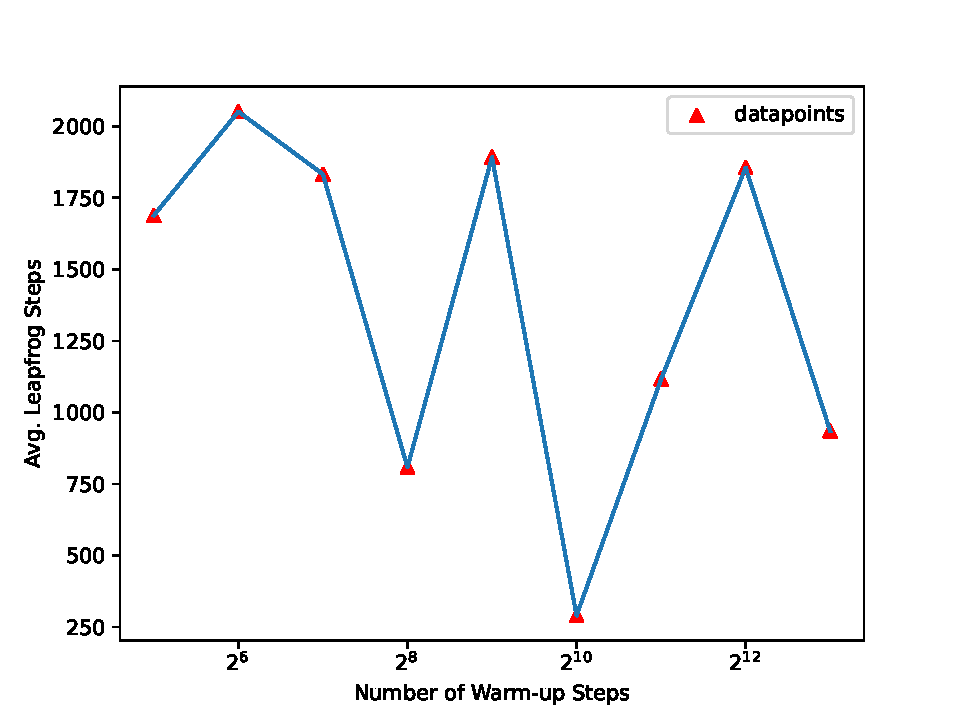
\includegraphics[scale=0.7]{figures/standardized_residuals/effect_of_burnin/avg_burnin_steps_nuts_vs_burn_in_steps.pdf}
    \caption{The figure shows the average number of Leapfrog steps $L$ as a function of number of warm-up steps used by the NUTS sampler when sampling the models shown in the bottom of figure \ref{fig:standardized_residuals_vs_burn_in_steps}. We have included a few more measurements to showcase how fluctuating the average number can be. 
    }
    \label{fig:avg_leapfrog_steps_vs_burn_in}
\end{figure}




\subsubsection{The Effect of Pretraining}
Pretraining a model before initiating the Markov chain is typically suggested as a means to accelerate convergence to the stationary distribution by minimizing a selected loss function with respect to the model parameters to obtain a point estimate. The point estimate is then used as the initial point of the Markov chain. This may help but as we discussed in chapter \ref{chap:mcmc}, the typical set, the set which we seek to sample from, may not lay particularly close to the mode of the loss function, or as we know it as, the potential energy function. Thus we have good reasons to challenge this recommendation and verify that it indeed improves the performance of the BNN models we sample. We trained a BNN model with the architechture 5-20-20-1 with $\tanh(x)$ as the activation function in the hidden layers. We fixed the number of warm-up steps to 1000 of which 800 were used for adaptation of the step size and 200 were used for burn-in. We fixed the number of Leapfrog steps to $L = 512$ using the HMC sampler. As usual, we sampled 1000 neural networks with 10 steps between each sampled network. From the figure, we can observe that the performance of the model increases as we increase the number of pretraining epochs which gives us empirical grounds for initiating the Markov chain from the point estimate obtained. As in the previous section, we see can not a dramatic decrease in performance when we transform the predictions back to target space and compute the $R^2$-score. 


In figure \ref{fig:std_residual_vs_pretraining}, we
show the computed standardized residuals in log space. The figure demonstrates a pretty noticable improvement as the amount of pretraining increases, up to a point. Once we surpass 2048 epochs of pretraining, we see a slight degradation of the model performance with a larger spread in the residual distribution. But we can rest assured that pretraining can be used to increase the performance of the trained BNN when everything else is held fixed, and should thus be applied as part of the training procedure. Note that the model used here consists of a rather small number of parameters. We performed pretraining of the models on a GPU which yielded less than 10\% GPU utilization, while the MCMC sampling of the model parameters required $\sim 90\%$ GPU utilization. Hence pretraining with models of this size is better performed on either a built-in GPU on an SoC such as the one shipped with an Apple Silicon SoC. Else, the pretraining should be employed on a multi-core CPU device.

\begin{figure}[h!]
    \centering
    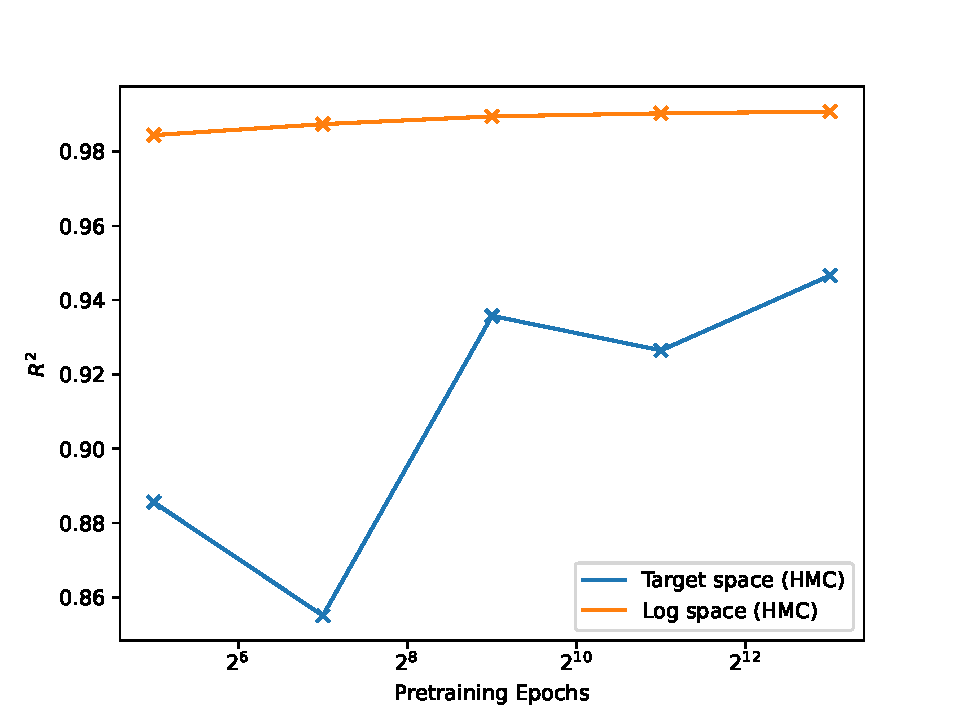
\includegraphics[scale=0.7]{figures/r2_scores/r2_score_vs_pretraining.pdf}
    \caption{The figure shows the computed $R^2$-scores of a model with the architecture 5-20-20-1 with $\tanh(x)$ as the
    hidden activation function. In this case the varying number of the number of epochs run with pretraining starting from 32 all the way up to 8192. The batch size used was 32 with the ADAM optimizer. The number of warm-up steps was 1000 (200 of which were burn-in steps and 800 were adaptation steps). We fixed the Leapfrog steps to $L = 512$ using the HMC sampler. As usual we sampled 1000 neural networks with 10 steps between each sample.
    }
    \label{fig:r2_score_vs_pretraining}
\end{figure}


\begin{figure}[h!]
    \centering
    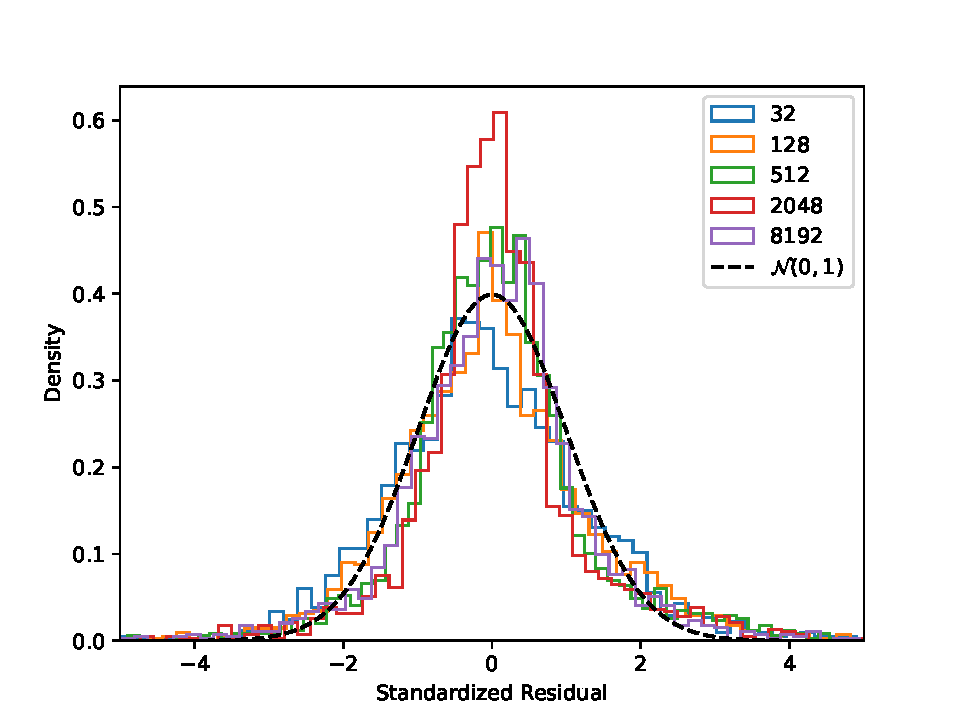
\includegraphics[scale=0.7]{figures/standardized_residuals/effect_of_pretraining/standardized_residuals_hmc_vs_pretraining_steps.pdf}
    \caption{The figure shows the standardized residuals of a model with the architecture 5-20-20-1 with $\tanh(x)$ as the
    hidden activation function. In this case the varying number of the number of epochs run with pretraining starting from 32 all the way up to 8192. The batch size used was 32, the number of warm-up steps was 1000 (200 of which were burn-in steps and 800 were adaptation steps). We fixed the Leapfrog steps to $L = 512$ using the HMC sampler. The ADAM optimizer was used for the pretraining phase. As usual we sampled 1000 neural networks with 10 steps between each sample.
    }
    \label{fig:std_residual_vs_pretraining}
\end{figure}

\subsubsection{Effect of Number of Parameters}
Increasing the number of parameters of the BNN model may help capture the underlying process from the data to a larger degree. The typical problems posed by the \textit{bias-variance trade-off} \cite{ml_for_physicists} (pages 12-13) does not play as significant a role here since the trained model can compute a sample variance along with its prediction. This does not mean it is immune, however, as the model is still sampled according to the nuances found in the training data which in principle may be due to noise. Moreover, the training data may not be particularly representive of the distribution of the underlying process we are trying to learn from the training data, or it may contain outlies which the model gathers samples to explain. As explained in section \ref{sec:perf_metrics}, the dataset produced by {\tt Prospino} contains very little noise and thus specializing the model to the inherent noise is not the issue. We did, however, see outliers in figure \ref{fig:dataset_masses} and figure \ref{fig:dataset_mixing_angles}. If a model has a large number of parameters, then, the training may produce a BNN model that generalizing poorly to the unseen test data because it attempts to account for the outliers. Moreover, the dataset we use is fairly small ($\sim 16000$ datapoints in total), which can exacerbate the effect.

In figure~\ref{fig:r2_scores_vs_num_params} we show the computed $R^2$ score on the training and test data as a function of number of nodes $n$ placed in the hidden layer of models with the architecture 5-$n$-1. The hidden activation used was $\tanh(x)$. The training was carried out with 1000 warm-up steps with the usual division of 20\% burn-in steps and 80\% allocated to adapdation of the step size in the Leapfrog integrator. We performed 2500 pretraining steps with a batch size of 32 for each model. When using the HMC sampler, we fixed the number of Leapfrog steps to $L = 512$. For the NUTS sampler, we allowed a maximum of $L = 4096$ Leapfrog steps. We sampled 1000 networks in each cases, skipping 10 networks between each stored sample. The models trained with the HMC sampler increase in performance up until a maximum after which the performance degrades, which may be explained by the fixed number of Leapfrog steps in an increasingly higher-dimensional parameter space. Moreover, the dataset used is fairly small for $7n + 1$ parameters in total as $n$ increases (which in the highest case of $n = 2^13 = 8192$ parameters imply 57345 parameters per sampled neural network). 

\begin{figure}[h!]
    \centering
    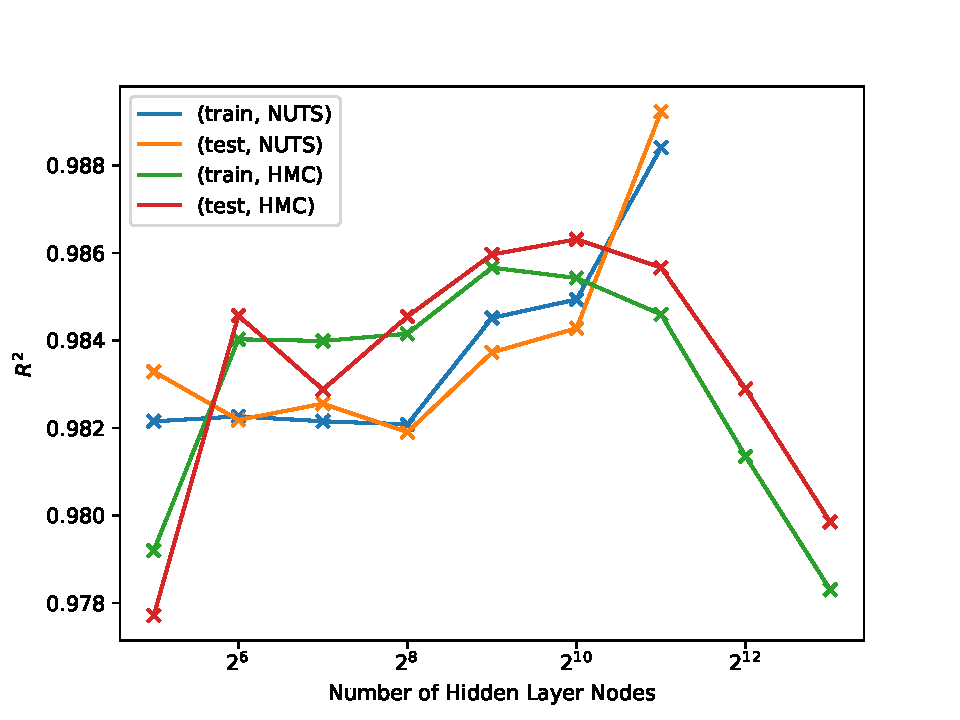
\includegraphics[scale=0.7]{figures/r2_scores/r2_score_vs_num_params_log_space.pdf}
    \caption{
        The figure shows the $R^2$-score computed on the training and test data as a function of number of nodes $n$ in the hidden layer of models with architechture 5-$n$-1, yielding a total of $5n + 1$ parameters. The hidden layer activation used was $\tanh(x)$.
        The models were trained with 1000 warm-up steps (20\% burn-in and 80\% adaptation), gathering 1000 neural networks with 10 steps between each sample. We used 2500 pretraining epochs with a batch size of 32. 
        When using the HMC sampler, we fixed the number of Leapfrog steps to $L = 512$. When using NUTS, we set a maximum of $L = 4096$ Leapfrog steps. 
    }\label{fig:r2_scores_vs_num_params}
\end{figure}



In figure \ref{fig:standardized_residual_vs_params}, we show the computed standardized residual distribution of the models listed in table \ref{tab:deep_models}, which gives us an idea of the performance the BNNs have on this dataset as a function of the number of parameters. We can note that model 3 and 4 performs fairly well given our chosen benchmark measure, but that model 5's performance degrade somewhat, which is the model that contains the most parameters of the models tested. 

\begin{figure}[h!]
    \centering
    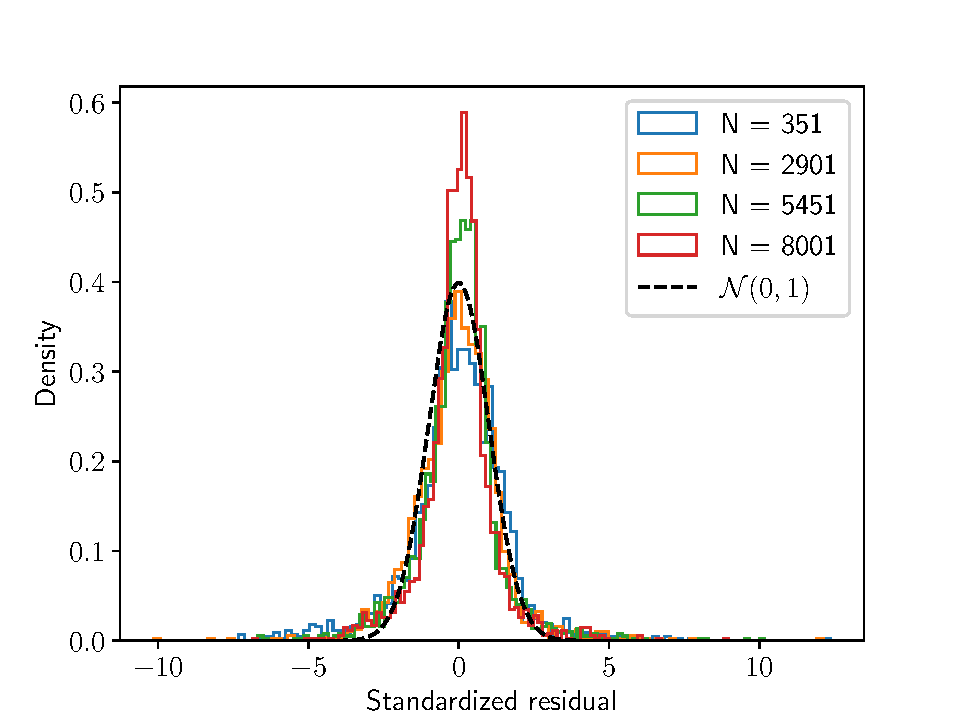
\includegraphics[scale=0.7]{figures/standardized_residuals/standardized_residual_simple_models.pdf}
    \caption{
        The figure shows the distribution of the standardized residuals computed on the test data using the models listed in table \ref{tab:deep_models}. The Normal distribution is drawn in with a dotted black line for benchmarking reference.
        The figure is meant to illustrate the performance of the models with respect to the number of parameters in the models.
        The models were trained with 2500 warm-up steps (20\% burn-in and 80\% adaptation), gathering 1000 neural networks with 10 steps between each sample. We used 1000 pretraining epochs with a batch size of 32. The kernel used was the NUTS kernel with a maximum of $L = 4096$ Leapfrog steps. 
    }
    \label{fig:standardized_residual_vs_params}
\end{figure}

\subsection{Predictive Distributions}
As we discussed in chapter \ref{chap:bayesian_ml}, one of the primary objects we seek to compute
in Bayesian ML is the predictive distribution $p(y^*|x^*, D)$ for a target $y^*$ given an unseen input point $x^*$ and
a training dataset $D$. In figure \ref{fig:predictive_distributions}, we show the predictive distribution computed with model 3 in table \ref{tab:deep_models}. In the figure on top, the sample mean approximates the true target well with a fairly small spread in the distribution which is a desirable outcome in most cases. There are, however, ill cases as well which we demonstrate in the figure at the bottom. Here the true target lies entirely outside the predictive distribution. Thus care must be taken to understand when a BNNs prediction is reliable and when it is not. We can deal with this problem by empirically counting how many targets $y \in [\mu - k\sigma, \mu + k \sigma]$ for $k = 1, 2, 3, 4, 5$ where $\mu$ represents the sample mean and $\sigma^2$ represents the sample variance of each predictive distribution computed by the BNN model. In principle there is no need for $k$ to be an integer, and a finite grid of points $k \in (0s, \infty)$ can be used instead such that an arbitrary desired accuracy can be specified. We illustrate the results of this analysis in figure \ref{fig:confidence} performed on the training, validation and test data. Clearly there exists a small percentage of ill cases where the target lies far away from the predicted mean. The result does at least tell us that more than 95\% of the targets lie within $\mu \pm 3\sigma$ over each dataset in their respective predictive distribution.
\begin{figure}[h!]
    \centering
    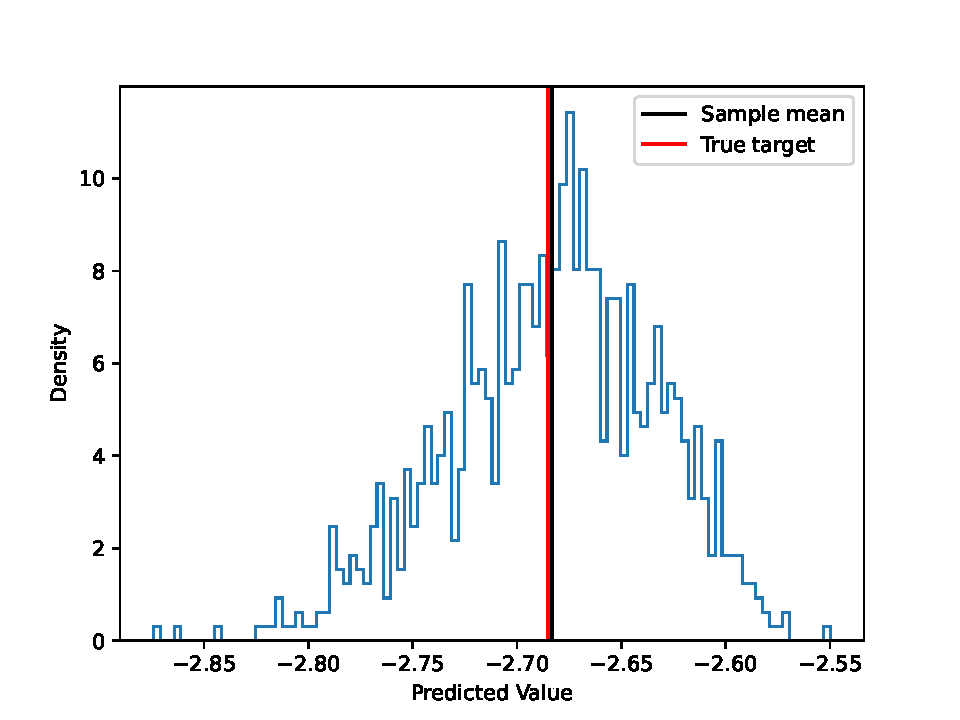
\includegraphics[scale=0.7]{figures/predictive_distributions/predictive_distribution_point_idx_360.pdf}
    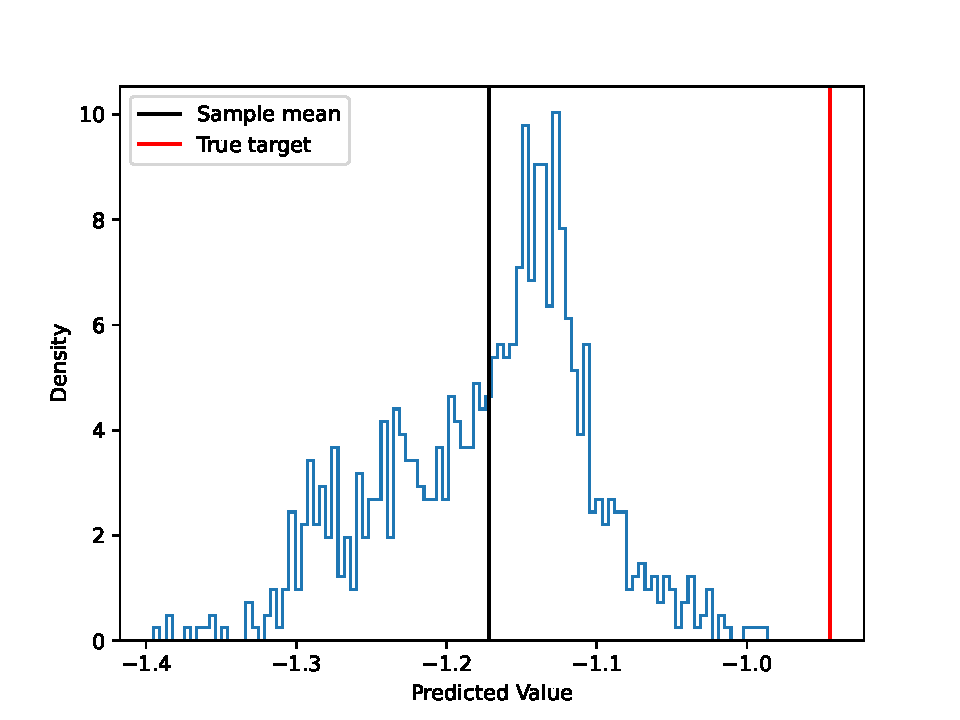
\includegraphics[scale=0.7]{figures/predictive_distributions/predictive_distribution_point_idx_2052.pdf}
    \caption{
        The figure shows the predictive distribution estimated by use of model 3 in table \ref{tab:deep_models} for to randomly chosen points from the test set. The red line shows the true target and the black line shows the predicted sample mean obtained from the distribution. The figure on top demonstrates a case where the sample mean is approximately the same as the target, while the figure at the bottom demonstrates a case where the true target lies entirely outside the predictive distrbution. 
    }
    \label{fig:predictive_distributions}
\end{figure}


\begin{figure}[h!]
    \centering
    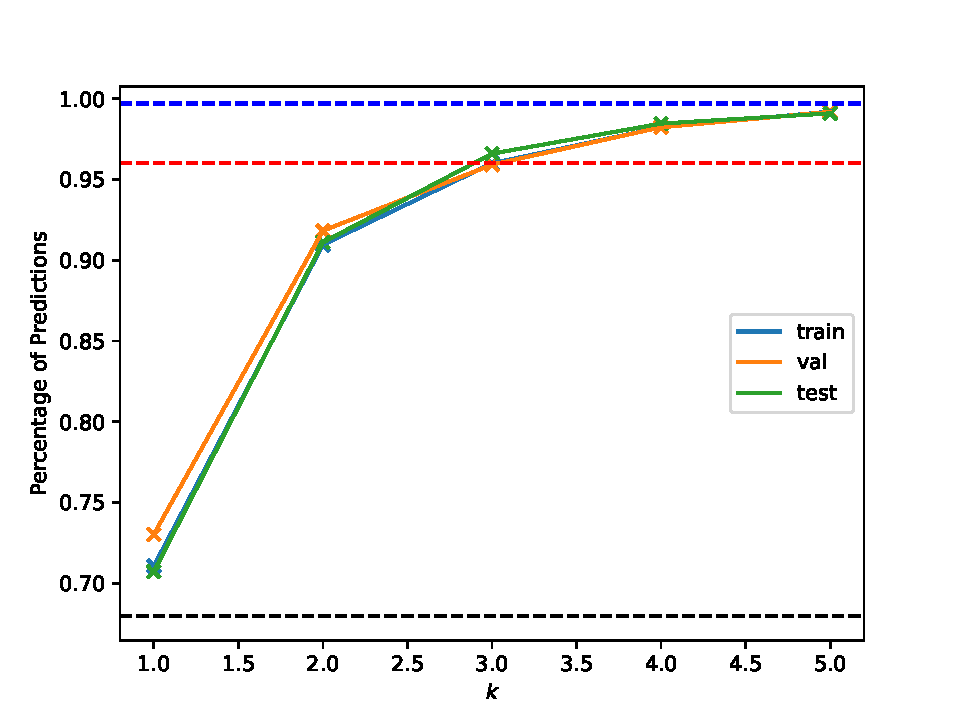
\includegraphics[scale=0.7]{figures/confidence_estimation/good_vs_bad_cases_confidence.pdf}
    \caption{
        The figure shows the predictive distribution estimated by use of model 3 in table \ref{tab:deep_models}
        computed on all datapoints in the training, validation and test data. The black line shows the 95\% line. The crosses indicate measured data with training data shown in blue, validation data shown in orange and test data shown in green. The $y$-axis shows the percentage of all targets lie on the interval $[\mu - k\sigma, \mu + k\sigma]$ for $k=1,2,3,4,5$ where $\mu$ is the sample mean and $\sigma^2$ is the sample variance of the predictive distribution.
    }
    \label{fig:confidence}
\end{figure}







